%% ----------------------------------------------------------------
%% Implement.tex
%% ----------------------------------------------------------------
\chapter{Implementation}

\section{Background subtraction}

\subsection{Colour based}

An simple implementation \cite{MOTBOC.git} of colour filtering object detection algorithm was investigated, as shown in \fref{Figure:MOTBOC}.

However, this implementation is very limited, it can only detects objects with single colour, cannot distinguishes the objects from similar background colour, relies heavily on manually adjusted colour threshold values, and is very sensitive to the variations of colourspaces from different cameras, not very adaptable. A complex environment may also results into lots of undesired detections, as shown in \fref{Figure:MOTBOC_F}.

\begin{figure}[H]
  \centering
  \includegraphics[width=0.6\columnwidth]{"MOTBOC failure"}
  \caption{Simple Multi Object Tracking Based on Color \cite{MOTBOC.git} at a complex environment}
  \label{Figure:MOTBOC_F}
\end{figure}

\subsection{Shape based}

OpenCV's implementation of Hough Circle Transform for circle detection was investigated. However, this algorithm is still very limited and inaccurate, as shown in \fref{Figure:circles}, the coin at the top right corner had not been detected, because it actually appeared to be a eclipse to the algorithm because of visual perspective. Furthermore, in order to detect multiple geometric shapes, a different algorithm would be required for each of the different shapes.

\subsection{Cascade Classifier}

Noticeable frame rate drop and latency was experienced when experiments with the cascade classifier implementation on the testing platform as shown in \fref{Figure:cc_face}, suggests it was not a fast enough algorithm for real-time object tracking application. In addition, multiple classifier definition files were required for detecting different kinds of objects, or even different perspectives of the same object, which would require lots of computations.

\subsection{Motion based}

The article \cite{bgs:article} reviewed the algorithms available in the BGSLibrary, ranked 5 algorithms as the best methods for accuracy. Except the Pixel-Based Adaptive Segmenter (PBAS) algorithm which was removed due to patent issues, the other 4 algorithms listed in \tref{Table:bgs} were investigated in this project.

\begin{table}[H]
  \centering
  \begin{tabular}{cc}
  \toprule
  \textbf{Method ID} & \textbf{Method name}\\
  \midrule
  MultiLayerBGS & Multi-Layer BGS \\
  MixtureOfGaussianV1BGS & Gaussian Mixture Model \\
  LBAdaptiveSOM & Adaptive SOM \\
  DPWrenGABGS & Gaussian Average \\
  \bottomrule
  \end{tabular}
  \caption{Background substraction algorithms investigated (adapted from \cite{bgslibrary})}
  \label{Table:bgs}
\end{table}

\fref{Figure:bgs_frame} shows the foreground masks obtained from those 4 algorithms through 2 sample frame sequences available with the BGSLibrary \cite{bgslibrary}.

\begin{figure}[H]
  \centering
  \includegraphics[width=0.24\columnwidth]{bgs_frame/MultiLayerBGS/input}
  \includegraphics[width=0.24\columnwidth]{bgs_frame/MultiLayerBGS/mask}
  %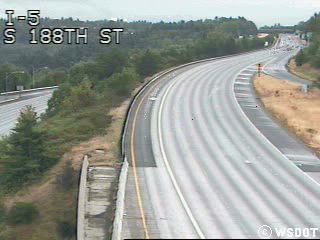
\includegraphics[width=0.32\columnwidth]{bgs_frame/MultiLayerBGS/bkgmodel}
  \includegraphics[width=0.24\columnwidth]{bgs_video/MultiLayerBGS/input}
  \includegraphics[width=0.24\columnwidth]{bgs_video/MultiLayerBGS/mask}

  \includegraphics[width=0.24\columnwidth]{bgs_frame/MixtureOfGaussianV1BGS/input}
  \includegraphics[width=0.24\columnwidth]{bgs_frame/MixtureOfGaussianV1BGS/mask}
  \includegraphics[width=0.24\columnwidth]{bgs_video/MixtureOfGaussianV1BGS/input}
  \includegraphics[width=0.24\columnwidth]{bgs_video/MixtureOfGaussianV1BGS/mask}
  %
\includegraphics[width=0.32\columnwidth]{na}

  \includegraphics[width=0.24\columnwidth]{bgs_frame/LBAdaptiveSOM/input}
  \includegraphics[width=0.24\columnwidth]{bgs_frame/LBAdaptiveSOM/mask}
  \includegraphics[width=0.24\columnwidth]{bgs_video/LBAdaptiveSOM/input}
  \includegraphics[width=0.24\columnwidth]{bgs_video/LBAdaptiveSOM/mask}
  %
\includegraphics[width=0.32\columnwidth]{na}

  \includegraphics[width=0.24\columnwidth]{bgs_frame/DPWrenGABGS/input}
  \includegraphics[width=0.24\columnwidth]{bgs_frame/DPWrenGABGS/mask}
  \includegraphics[width=0.24\columnwidth]{bgs_video/DPWrenGABGS/input}
  \includegraphics[width=0.24\columnwidth]{bgs_video/DPWrenGABGS/mask}
  %
\includegraphics[width=0.32\columnwidth]{na}
  \caption{Results obtained from background substraction algorithms. From left to right column: input sample 1, foreground mask obtained, input sample 2, foreground mask obtained. From top to bottom row: MultiLayerBGS, MixtureOfGaussianV1BGS, LBAdaptiveSOM and DPWrenGABGS.}
  \label{Figure:bgs_frame}
\end{figure}

It can be seen from \fref{Figure:bgs_frame} that MultiLayerBGS gave the best foreground masks, but it was also the slowest algorithm on the testing platform.

\section{Movement tracking}

This was not yet implemented at the time this progress report was written.
